\section[Выбор и обоснование средств реализации]{ВЫБОР И ОБОСНОВАНИЕ \\ СРЕДСТВ РЕАЛИЗАЦИИ}
\label{sec:choice}

\subsection{Язык программирования}

Целью данного курсового проекта является написание архиватора.
Архиватор --- системное ПО, следовательно, для его написания желательно
использовать соответствующий язык программирования, 
чтобы программа, написанная на нем, обладала следующими свойствами:

\begin{itemize}
\item имела высокую производительность;
\item была переносимой;
\item была достаточно простой для понимания.
\end{itemize}

Поясним эти требования.

\textit{Высокая производительность} чрезвычайно важна для архиватора,
так как на практике нередко требуется сжимать большие файлы,
причем желательно делать это за минимально возможное время.

\textit{Переносимость} означает способность программы работать на
компьютерных системах с различной архитектурой и под управлением 
различных операционных систем.

Под \textit{простотой для понимания} имеется в виду как относительная 
популярность, так и простота синтаксических конструкций языка программирования.

Кроме этого, есть еще одно дополнительное требование:
в языке должна быть предусмотрена \textit{возможность работы с отдельными битами}.
Дело в том, что результатом кодирования Хаффмана является набор кодов 
переменной длины, которые могут занимать нецелое число байт. 

Исходя из вышеперечисленных требований, в качестве языка реализации
архиватора был выбран язык программирования C.

C --- компилируемый статически типизированный язык программирования общего
назначения, разработанный в 1969--1973 годах сотрудником Bell Labs
Деннисом Ритчи как развитие языка B.
Первоначально был разработан для реализации операционной системы UNIX,
но, впоследствии, был перенесён на множество других платформ.
Благодаря близости по скорости выполнения программ, написанных на C,
к языку ассемблера, этот язык получил широкое применение при создании
системного программного обеспечения и прикладного программного
обеспечения для решения широкого круга задач~\cite{wiki_c}.

Перечислим его основные достоинства:
\begin{itemize}
\item компилируемый --- при компиляции программы из исходных кодов
  компилятор производит различные оптимизации машинного кода, 
  тем самым увеличивая производительность;
\item статически типизируемый --- при выполнении программы, написанной на C,
  не затрачивается времени на определение типа переменных,
  что положительно сказывается на быстродействии;
\item переносимый --- код, написанный в соответствии со стандартом ANSI C,
  гарантированно может быть откомпилирован и запущен в среде с 
  соответствующей реализацией стандарта~\cite{ansi_c};
\item популярный --- по данным ресурса langpop.com~\cite{langs_popularity},
  язык программирования С является самым известным языком программирования 
  общего назначения.
\end{itemize}

Таким образом, можно сделать вывод, что язык программирования C идеально 
подходит для написания разрабатываемого ПО в рамках данного курсового проекта. 

\subsection{Система сборки проекта}
\label{ssec:choice_build_system}

\textit{Система сборки проекта} --- программа, выполняющая сборку, 
запуск и тестирование приложения на основании некоторых правил,
определяемых программистом. 
Система сборки проекта используется для упрощения рутинного процесса сборки 
и тестирования разрабатываемой программы.

В качестве системы сборки разрабатываемого проекта была выбрана утилита GNU Make.

GNU Make --- утилита, автоматизирующая процесс преобразования файлов
из одной формы в другую.

Данный выбор обусловлен следующими причинами:
\begin{itemize}
\item GNU Make является стандартной утилитой сборки проектов,
  написанных на C;
\item GNU Make использует простой и понятный декларативный синтаксис для
  описания целей сборки;
\item GNU Make присутствует в репохиториях кждого дистрибутива GNU/Linux, *BSD,
  а также есть в наборах утилит Cygwin и MinGW, используемых под Windows;
\item работа GNU Make не ограничивается компиляцией исходных файлов,
  она может использоваться для выполнения практически любых задач,
  требуемых для сборки (генерация документации, запуск тестов, \dots);
\item GNU Make --- свободное программное обеспечение,
  созданное в рамках проекта GNU.
\end{itemize}

Немаловажным фактом при выборе системы сборки в пользу GNU Make 
послужило наличие подробной документации на официальном сайте 
проекта~\cite{doc_make}.

\subsection{Система контроля версий}

\textit{Система контроля версий} --- программное обеспечение для облегчения
работы с изменяющейся информацией.
При разработке программного обеспечения систему контроля версий использовать
для хранения нескольких версий одних и тех же файлов исходного кода,
обеспечения независимости разработки отдельных частей,
возврата при необходимости к более ранним версиям кода.

В качестве системы контроля версий разрабатываемого программного обеспечения
был выбран git.

Git --- распределённая система контроля версий файлов.
Термин <<распределенная>> означает, что при клиенты данной системы при
клонировании данных не просто получают последнюю версию,
а полностью копируют весь репозиторий.
Это играет решающую роль в тех случаях, когда отказывает 
общий сервер, хранящий репозиторий. 
В таком случае после восстановления работоспособности сервера данные
на нем могут быть восстановлены с репозитория,
находящегося у любого из клиентов, как показано на рисунке~\ref{pic:git}.

Кроме того, в большей части этих систем можно работать с несколькими
удалёнными репозиториями, таким образом, можно одновременно работать по-разному
с разными группами людей в рамках одного проекта.
Так, в одном проекте можно одновременно вести несколько типов рабочих процессов,
что невозможно в централизованных системах~\cite{doc_scm}.

\begin{figure}[h!]
  \centering
  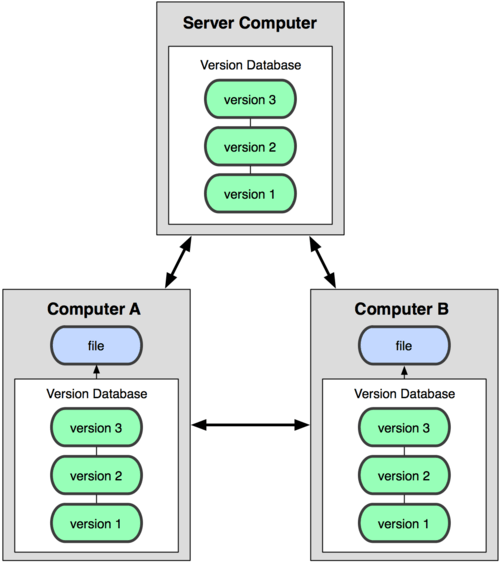
\includegraphics[width=150mm]{pic/git.png}
  \caption{Схема распределенной системы контроля версий}
  \label{pic:git}
\end{figure}

Также немаловажно отметить факт существования публичного сервиса github.com,
который предоставляет возможность бесплатного хранения репозиториев
с открытым исходным кодом.

\subsection{Генератор документации}

\textit{Генератор документации} --- программа или пакет программ, 
позволяющая получать документацию, предназначенную для программистов
(документация на API) и/или для конечных пользователей системы,
по особым образом комментированному исходному коду и,
в некоторых случаях, по исполняемым модулям (полученным на выходе компилятора).

Обычно генератор анализирует исходный код программы,
выделяя синтаксические конструкции, соответствующие значимым объектам программы 
(типам, классам и их членам/свойствам/методам, процедурам/функциям и т. п.).
В ходе анализа также используется мета-информация об объектах программы,
представленная в виде документирующих комментариев. 
На основе всей собранной информации формируется готовая документация, 
как правило, в одном из общепринятых форматов — HTML, HTMLHelp, PDF, 
RTF и других.

Для генерирования документации на основе исходного кода разрабатываемого проекта
была выбрана утилита doxygen. 

Doxygen --- кроссплатформенная система документирования исходных текстов,
которая поддерживает C++, С, Objective-C, Python, Java, IDL, PHP, C\#, Fortran,
VHDL.

Doxygen --- консольная программа в духе классической Unix.
Она работает подобно компилятору, анализируя исходные тексты и создавая
документацию. Параметры создания документации читаются из конфигурационного 
файла, имеющего простой текстовый формат~\cite{gen_doc}.
Данная особенность обеспечивает легкую интеграцию Doxygen с GNU Makefile.
